We consider a traffic signal control application where the aim is to improve the road user experience by an adaptive traffic light control (TLC) algorithm.
We adopt a CPT approach, i.e., apply the CPT-functional to the delay experienced by road users. We then optimize the CPT-value of the delay  and contrast this approach with a traditional expected delay optimizing algorithm.

%\paragraph{Simulation Setup:}  
We consider a road network with $\N$ signalled lanes that are spread across junctions and $\M$ paths, where each path connects (uniquely) two edge nodes, where the traffic is generated - see Figure \ref{fig:2x2grid}.
At any instant $n$, let $q_n^i$ and $t_n^i$ denote the queue length and elapsed time since the lane turned red, for any lane $i = 1,\ldots, \N$. Let $d_n^{i,j}$ denote the delay experienced by $j$th road user on $i$th path, for any $i=1,\ldots,\M$ and $j=1,\ldots,n_i$, where $n_i$ denotes the number of road users on path $i$.
We specify the various components of the traffic control MDP in the following.
The state $s_n=(q_n^1,\ldots,q_n^{\N},t_n^1,\ldots,t_n^{\N},d_n^{1,1},\ldots,d_n^{\M,n_{\M}})\tr$ is a vector of lane-wise queue lengths, elapsed times and path-wise delays.
The actions are the feasible sign configurations that specify red-green combinations for the traffic lights in the road network considered. 

We consider three different notions of return as described below:

\textbf{CPT:} Let $\mu^i$ be the proportion of road users along path $i$, for $i=1,\ldots,\M$. Any road user along path $i$, will evaluate the delay he experiences in a manner that is captured well by CPT. Let $X_i$ be the delay r.v. for path $i$ and let the corresponding CPT-value be $\C(X_i)$. With the objective of maximizing the experience of road users across paths, the overall return to be optimized is given by\\[1ex]
\centerline{$\text{CPT}(X_1,\ldots,X_{\M}) = \sum_{i=1}^{\M} \mu^i \C(X_i).
$}

\textbf{EUT:} Here we only use the utility functions $u^+$ and $u^-$ to handle gains and losses, but do not distort probabilities. 
Thus, the EUT objective is defined as
\begin{align}
\text{EUT}(X_1,\ldots,X_{\M}) = \sum_{i=1}^{\M} \mu^i \left(\E(u^+(X_i) - \E(u^-(X_i)\right),
\end{align}   
where $\E(u^+(X_i)) = \intinfinity P(u^+(X_i)>z) dz$ and $\E(u^-(X_i)) - \intinfinity P(u^-(X_i)>z) dz$, for $i=1,\ldots,\M$.

\textbf{AVG:} This is similar to EUT, except that no distinction between gains and losses via utility functions nor distort using weights as in CPT. Thus, $\text{AVG}(X_1,\ldots,X_{\M}) = \sum_{i=1}^{\M} \mu^i \E(X_i)$. 
%Thus, the AVG objective is defined as
%\begin{align}
%\text{AVG}(X_1,\ldots,X_{\M}) = \sum_{i=1}^{\M} \mu^i \E(X_i).
%\end{align}   
%where $\E(X_i) = \intinfinity P(u^+(X_i)>z) dz - \intinfinity P(u^-(X_i)>z) dz$.

An important concept in CPT is to employ a reference point to calculate gains and losses. Choosing a suitable reference point is challenging, but \cite{tversky1992advances} advocate using status-quo as the reference point. In our traffic control setting, we use path-wise delays obtained from a pre-timed TLC (cf. the Fixed TLCs in \cite{prashanth2011reinforcement}) as the reference point. In other words, if the delay of any algorithm (say CPT-SPSA) is less than that of pre-timed TLC, then the (positive) difference in delays is perceived as a gain and in the complementary case, the delay difference is perceived as a loss. The $d_n^{i,j}$ in the state $s_n$ are to be understood as the delay difference to the pre-timed TLC.  

The underlying policy in all the algorithms that we implement follows a Boltzmann distribution and has the form
\begin{equation}
\pi_{\theta}(s,a) = \frac{e^{\theta^{\top} \phi_{s,a}}}{\sum_{a' \in {\A(s)}} e^{\theta^{\top} \phi_{s,a'}}},
\hspace{6pt} \forall s \in \S,\;\forall a \in \A(s).
\label{eq:pi-boltzmann}
\end{equation}	
We employ the features proposed in \cite{prashanth2012threshold}, as the road network considered is high-dimensional (state space cardinality $> 10^{60}$). 

We implement the following TLC algorithms:

{\bf\em CPT-SPSA}: This is the first-order algorithm with SPSA-based gradient estimates, as described in Algorithm \ref{alg:1spsa}. In particular, the estimation scheme in Algorithm \ref{alg:holder-est} is invoked to estimate $\C(X_i)$ for each path $i=1,\ldots,\M$, with $d_n^{i,j}, j=1,\ldots,n_i$ as the samples.

{\bf\em EUT-SPSA}: This is similar to CPT-SPSA, except that weight functions $w^+(p)=w^-(p)=p,$ for $p\in [0,1]$. 

{\bf\em AVG-SPSA}: This is similar to CPT-SPSA, except that weight functions $w^+(p)=w^-(p)=p,$ for $p\in [0,1]$. 

For both CPT-SPSA and EUT-SPSA, the utility functions (see \eqref{eq:cpt-general}) are chosen as follows:
$u^+(x) =  |x|^{\sigma}$, and  $u^-(x) = \lambda |x|^{\sigma}$, with $\lambda = 2.25$ and $\sigma = 0.88$.
For CPT-SPSA, the weights are chosen as follows:
$w^+(p) = \frac{p^{\eta_1}}{{(p^{\eta_1}+ (1-p)^{\eta_1})}^{\frac{1}{\eta_1}}}$ and  
$w^-(p) = \frac{p^{\eta_2}}{{(p^{\eta_2}+ (1-p)^{\eta_2})}^{\frac{1}{\eta_2}}}$, with
$\eta_1 = 0.61$ and $\eta_2 = 0.69$, . These choices are based on median estimates given by \cite{tversky1992advances} and have been used earlier in a traffic application (see \cite{gao2010adaptive}).

We run each algorithm for $200$ iterations, where each iteration is composed of a two perturbed simulations, each of trajectory length $500$. After this phase, we fix the the policy is fixed for each algorithm and run $100$ independent simulations of the MDP (each with a trajectory length of $1000$). The overall CPT-value is estimated using path-wise $\C(X_i)$ and the results are plotted in Figure \ref{fig:histogram-perf}. For all the algorithms, we set $\delta_n = 1.9/n^{0.101}$ and $a_n = 1/(n+50)$ and this is motivated by standard guidelines - see \cite{spall2005introduction}. Further, for all algorithms, the initial point $\theta_0$ is the $d=32$-dimensional vector of ones and the operator $\Gamma_i$ projects $\theta_i$ onto the set $[0.1, 10.0]$, for $i=1,\ldots,d$.
    
%\paragraph{Results:} 
Figures \ref{fig:avg}--\ref{fig:cpt} present the histogram of the CPT-value computed for AVG-SPSA, EUT-SPSA and CPT-SPSA, respectively.  It is evident that both AVG-SPSA and EUT-SPSA perform poorly in comparison to CPT-SPSA, thus making apparent the need for specialized algorithms that incorporate CPT-based criteria.


 \begin{figure}[t]
    \centering
     \begin{tabular}{c}
\subfigure[2x2-grid network]{
\label{fig:2x2grid}
        \includegraphics[width=2.2in,height=1.2in]{fig/2x2grid.pdf}
}
\\		
\subfigure[AVG-SPSA]{
\label{fig:avg}
%\hspace{2em} 
\tabl{c}{\scalebox{0.7}{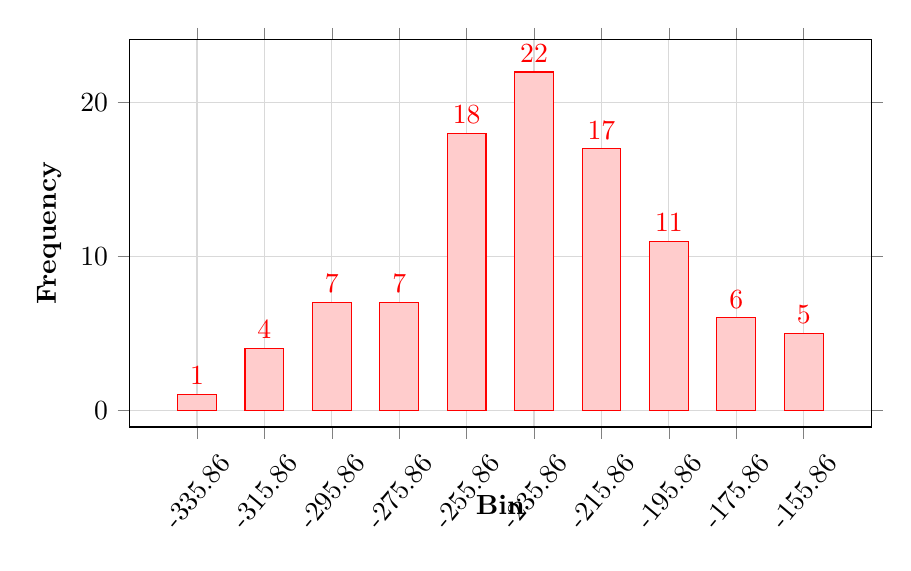
\begin{tikzpicture}
\begin{axis}[
ybar={2pt},
%  legend style={at={(0.5,-0.2)},anchor=north,legend columns=-1},
legend pos=outer north east,
legend image code/.code={\path[fill=white,white] (-2mm,-2mm) rectangle
(-3mm,2mm); \path[fill=white,white] (-2mm,-2mm) rectangle (2mm,-3mm); \draw
(-2mm,-2mm) rectangle (2mm,2mm);},
ylabel={\bf Frequency},
xlabel={\textbf{Bin}},
x label style={at={(axis description cs:0.5,-0.15)},anchor=north},
symbolic x coords={0, -335.86, -315.86, -295.86, -275.86, -255.86, -235.86, -215.86, -195.86, -175.86, -155.86, 11},
xmin={0},
xmax={11},
xtick=data,
ytick align=outside,
%xticklabels={{\bf7x9-Grid\\[0.5ex]($d=504$),\bf 14x9-Grid\\[0.5ex]($d=1008$),\bf 14x18-Grid\\[0.5ex]($d=2016$),\bf 28x18-Grid\\[0.5ex]($d=4032$)}},
xticklabel style={rotate=50, align=center},
bar width=14pt,
nodes near coords,
grid,
grid style={gray!30},
width=11cm,
height=6.5cm,
]
\addplot[red, fill=red!20]   coordinates {  (-335.86,1) (-315.86,4) (-295.86,7) (-275.86,7) (-255.86,18) (-235.86,22) (-215.86,17) (-195.86,11) (-175.86,6) (-155.86,5)}; %LSPI
\end{axis}
\end{tikzpicture}}\\[1ex]}
}
\\
%%%%%%%%%%%%%%
\subfigure[EUT-SPSA]{
\label{fig:eut}
%\hspace{2em} 
\tabl{c}{\scalebox{0.7}{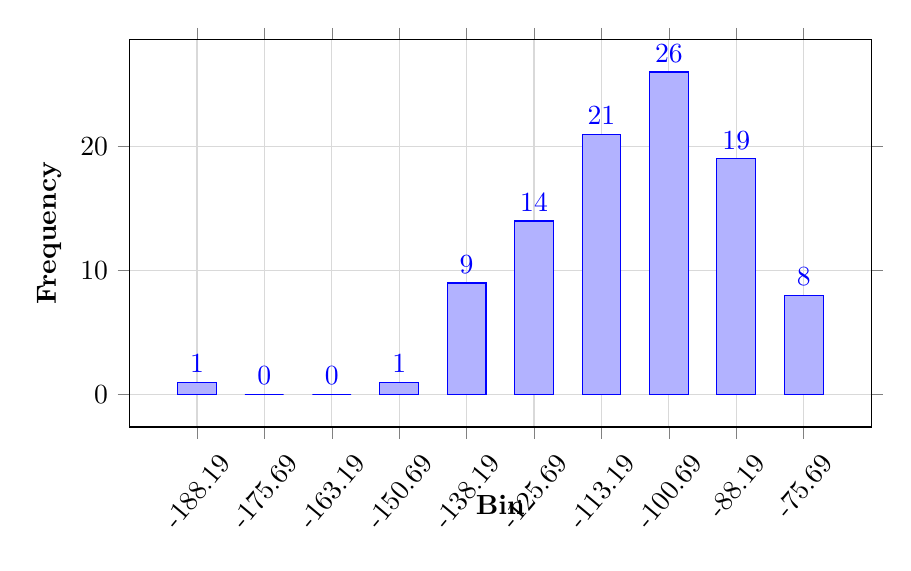
\begin{tikzpicture}
\begin{axis}[
ybar={2pt},
%  legend style={at={(0.5,-0.2)},anchor=north,legend columns=-1},
legend pos=outer north east,
legend image code/.code={\path[fill=white,white] (-2mm,-2mm) rectangle
(-3mm,2mm); \path[fill=white,white] (-2mm,-2mm) rectangle (2mm,-3mm); \draw
(-2mm,-2mm) rectangle (2mm,2mm);},
ylabel={\bf Frequency},
xlabel={\textbf{Bin}},
x label style={at={(axis description cs:0.5,-0.15)},anchor=north},
symbolic x coords={0,-188.19,-175.69,-163.19,-150.69,-138.19,-125.69,-113.19,-100.69,-88.19,-75.69,11},
xmin={0},
xmax={11},
xtick=data,
ytick align=outside,
%xticklabels={{\bf7x9-Grid\\[0.5ex]($d=504$),\bf 14x9-Grid\\[0.5ex]($d=1008$),\bf 14x18-Grid\\[0.5ex]($d=2016$),\bf 28x18-Grid\\[0.5ex]($d=4032$)}},
xticklabel style={rotate=50, align=center},
bar width=14pt,
nodes near coords,
grid,
grid style={gray!30},
width=11cm,
height=6.5cm,
]
\addplot   coordinates {  (-188.19,1) (-175.69,0) (-163.19,0) (-150.69,1) (-138.19,9) (-125.69,14) (-113.19,21) (-100.69,26) (-88.19,19) (-75.69,8) }; %LSPI
\end{axis}
\end{tikzpicture}}\\[1ex]}
}
\\
%%%%%%%%%%%%%%%%%%%%%%%%%
\subfigure[CPT-SPSA]{
\label{fig:cpt}
%\hspace{2em} 
\tabl{c}{\scalebox{0.7}{\begin{tikzpicture}
\begin{axis}[
ybar={2pt},
%  legend style={at={(0.5,-0.2)},anchor=north,legend columns=-1},
legend pos=outer north east,
legend image code/.code={\path[fill=white,white] (-2mm,-2mm) rectangle
(-3mm,2mm); \path[fill=white,white] (-2mm,-2mm) rectangle (2mm,-3mm); \draw
(-2mm,-2mm) rectangle (2mm,2mm);},
ylabel={\bf Frequency},
xlabel={\textbf{Bin}},
x label style={at={(axis description cs:0.5,-0.15)},anchor=north},
symbolic x coords={0, -43.36,-33.36,-23.36,-13.36,-3.36,6.64,16.64,26.64,36.64,46.64, 11},
xmin={0},
xmax={11},
xtick=data,
ytick align=outside,
%xticklabels={{\bf7x9-Grid\\[0.5ex]($d=504$),\bf 14x9-Grid\\[0.5ex]($d=1008$),\bf 14x18-Grid\\[0.5ex]($d=2016$),\bf 28x18-Grid\\[0.5ex]($d=4032$)}},
xticklabel style={rotate=50, align=center},
bar width=14pt,
nodes near coords,
grid,
grid style={gray!30},
width=11cm,
height=6.5cm,
]
\addplot[darkgreen, fill=darkgreen!20]   coordinates {  (-43.36,1) (-33.36,0) (-23.36,0) (-13.36,1) (-3.36,0) (6.64,1) (16.64,8) (26.64,52) (36.64,24) (46.64,12) }; %LSPI
\end{axis}
\end{tikzpicture}}\\[1ex]}
}
\end{tabular}
\caption{Histogram of CPT-value of the average delay for three different algorithms (all based on SPSA): AVG uses plain sample means (no utility/weights), EUT uses utilities but no weights and CPT uses both utilites and weights.}
\label{fig:histogram-perf}
\end{figure}

